\documentclass[10.75pt,a4paper,openright,bottom=2cm]{article}
\usepackage[english]{babel}
\usepackage[T1]{fontenc} 
\usepackage[utf8]{inputenc}
\usepackage{graphicx}
\usepackage{auto-pst-pdf} 
\usepackage{float}
\usepackage{graphicx}
\usepackage{wrapfig}
\usepackage{subcaption}
\usepackage{textcomp}
\usepackage{geometry}
\usepackage{pdfpages}
\usepackage{amsmath}
\usepackage{amsfonts}
\usepackage{wrapfig}
\usepackage{lipsum} 
\usepackage{fancyhdr}
\usepackage{amsmath}
\usepackage{graphicx}
\usepackage{tcolorbox}
\usepackage{bbm}
\usepackage{braket}
\usepackage{amssymb}
\usepackage{pifont}
\newcommand{\cmark}{\ding{51}}%
\newcommand{\xmark}{\ding{55}}%
\usepackage[table]{xcolor, colortbl}
\usepackage{cancel}
\DeclareMathAlphabet{\pazocal}{OMS}{zplm}{m}{n}
\usepackage[colorlinks=true, allcolors=blue]{hyperref}
\usepackage{multicol}
\usepackage{physics}
\usepackage[super]{nth}
\usepackage{bbm}
\usepackage{tikz}
\usepackage[compat=1.1.0]{tikz-feynman}
\usetikzlibrary{positioning}
\usepackage{circuitikz}
\usetikzlibrary{arrows,shapes,positioning}
\usepackage{subfig}
\newcommand{\beginbox}[1]{\begin{tcolorbox}[width=\textwidth,colback={black!40},title={#1},colbacktitle={purple!55},coltitle=black]}
\renewcommand{\endbox}{\end{tcolorbox}\noindent}
% \begin{tcolorbox}[width=\textwidth,colback={yellow!50},title={Rosenbluth Cross Section},colbacktitle={gray!50},coltitle=black]
\title{\textbf{Neutrinos and Dark Matter}}
\author{Matteo D'Errigo}

% \begin{titlepage}
%    \begin{center}
%        \vspace*{1cm}

%        \textbf{Thesis Title}

%        \vspace{0.5cm}
%         Thesis Subtitle
            
%        \vspace{1.5cm}

%        \textbf{Author Name}

%        \vfill
            
%        A thesis presented for the degree of\\
%        Doctor of Philosophy
            
%        \vspace{0.8cm}
     
%        \includegraphics[width=0.4\textwidth]{university}
            
%        Department Name\\
%        University Name\\
%        Country\\
%        Date
            
%    \end{center}
% \end{titlepage}

\begin{document}
\maketitle
\tableofcontents
% \begin{abstract}
% \end{abstract}
\newpage
\section{Cosmology}
We know that the universe is expanding so the question is: \textit{is it accelerating?} We can answer this question by using the \textbf{comoving coordinates}, defining with $r$ the comoving distance. Moreover, we introduce a \textbf{scale factor} $a(t)$ which defines how the space expands and contracts. Therefore, the distance between the two objects is given by:
\[
d(t)=r\cdot a(t)\to\Dot{d}(t)=r\cdot\Dot{a}(t)
\]
Putting these two expressions together gives us:
\beginbox{Hubble Constant}
\[
v(t):=\Dot{d}(t)=\frac{\Dot{a}(t)}{a(t)}d(t)=H(t)d(t)
\]
\endbox
Where we have defined the ratio $\frac{\Dot{a}(t)}{a(t)}$ as the \textbf{Hubble constant} $H(t)$ (although it is \textit{not} really constant). At a reference time $t_0$ chosen to be today, it is possible to compute the value of the Hubble constant:
\[
v(t_0)=H_0\cdot d(t_0)\to H_0=68\,\text{km/(Mpc$\cdot$s)}=2\cdot10^{-18}\,\text{s$^{-1}$}
\]
Knowing now the value of $H_0$, it is then possible to solve the differential equation\\
$\Dot{d}(t_0)=H_0\cdot d(t_0)$, which gives us:
\[
d(t)=d(t_0)\exp{H_0(t-t_0)}\simeq d(t_0)[1+H_0(t-t_0)]
\]
where we have performed a first order approximation since $H_0$ is small. Moreover, we can also see how the volume increases:
\[
V(t)=V(t_0)\exp{3H_0(t-t_0)}\simeq V(t_0)[1+3H_0(t-t_0)]
\]
Taking now the ratio of these two expressions allows us to compute the \textbf{Hubble time}.
\beginbox{Hubble Time}
\[
t_H:=\frac{1}{H_0}=\frac{d(t_0)}{V(t_0)}=14.4\,\text{Gy}
\]
\endbox
This value is really close to the actual age of the Universe, 13.7 Gy. This discrepancy can be explained by considering the fact that the Hubble constant was greater in the past.\\
If we compute the distance that light has travelled during this time, we end up with:
\[
d(t_0)=c\cdot t_H=\frac{c}{H_0}=4300\,\text{Mpc}
\]
Light is not fast enough to reach objects from this distance. However, this is not in contrast with relativity because at this distance objects cannot \textit{talk} to each other. This distance tells us the size of what we can see in the Universe.\\
A phenomenon strictly related to the Hubble constant is the one of \textbf{redshift}:
\[
Z=\frac{\lambda_{\text{obs}}-\lambda_{\text{e}}}{\lambda_{\text{e}}}
\]
The scale factor $a(t_0)$ today is, by definition, 1, hence:
\[
\lambda_{\text{obs}}=\lambda_{\text{e}}\frac{a(t_0)}{a(t_{\text{e}})}
\]
The scale factor $a(t_{\text{e}})$ is smaller than 1 so today we observe longer wavelengths with respect to the time of their emission. It is possible to obtain a relation between the redshift and the scale factor. To do that, start with rewriting $Z$ as follows:
\[
Z=\frac{\lambda_{\text{obs}}}{\lambda_{\text{e}}}-1=\frac{a(t_0)}{a(t_{\text{e}})}-1=\frac{1}{a(t_{\text{e}})}-1
\]
Moreover, we know that $d(t)=r\cdot a(t)$, from which we can write:
\[
a(t)=a(t_0)[1+H_0(t-t_0)]=1+H_0(t-t_0)\to\frac{1}{a(t_{\text{e}})}=\frac{1}{1+H_0(t_{\text{e}}-t_0)}\simeq1-H_0(t_{\text{e}}-t_0)
\]
Therefore, at first order in our expansion we have:
\beginbox{Redshift}
\[
Z=H_0(t_0-t_{\text{e}})
\]
\endbox
Typically, what is observed is light for which it holds true that:
\[
d=c\Delta t=\frac{Zc}{H_0}
\]
This is how the Hubble constant was firstly measured.\\
With all this machinery, our goal is now to derive the \textbf{Friedmann equation}. Suppose to have a test mass $m$ on the edge of a sphere with radius $R$ which encloses a total mass $M$. The dynamics of the test mass is:
\[
m\Ddot{R}(t)=-G\frac{mM}{R^2(t)}
\]
We are interested in $\Ddot{R}(t)$ which is the acceleration per unit mass. Take into account now the \textbf{energy density}, defined as follows:
\[
\varepsilon=\int dt\Ddot{R}(t)\Dot{R}(t)=\int d\Dot{R}\Dot{R}(t)=\frac{\Dot{R}^2}{2}
\]
However, we can express $\Ddot{R}(t)$ from the dynamics of the test mass, resulting in:
\[
\varepsilon=\int dt\left(-G\frac{M}{R^2(t)}\right)\Dot{R}(t)=-GM\int \frac{dR}{R^2(t)}=\frac{GM}{R(t)}\Rightarrow\frac{\Dot{R}^2}{2}=\frac{GM}{R(t)}+U
\]
We take a look at the possible values of $U$:
\begin{itemize}
    \item $U>0$: the object escapes the gravitational force since $\Dot{R}(0)>$\,escape velocity
    \item $U=0$: $\Dot{R}(0)=$\,escape velocity
    \item $U<0$: $\Dot{R}(0)<$\,escape velocity
\end{itemize}
At this point we have to take into account that the sphere we are considering might change its volume and density, assuming that the total mass $M$ stays fixed:
\[
M=\frac{4}{3}\pi R^3(t)\rho(t)\to\Dot{R}^2=R_0^2\Dot{a}^2(t)=\frac{8}{3}\pi G\rho(t)R_0^2a^2(t)+2U
\]
where we used the fact that $R(t)=R_0a(t)$. Last thing left to do is to divide both sides by $R_0^2a^2(t)$ which gives us:
\beginbox{Friedmann Equation (classical derivation)}
\[
H^2(t)=\left(\frac{\Dot{a}(t)}{a(t)}\right)^2=\frac{8}{3}\pi G\rho(t)+\frac{2U}{R_0^2a^2(t)}
\]
\endbox
What we have done so far was a classical treatment, now we move to the relativistic case where the energy density can be expressed as $\varepsilon(t)=\rho(t)c^2$. The tricky part comes when we have to define the initial conditions, which were simply given by the factor proportional to $U$ in the previous formulation. Working with \textbf{Minkowski metric}, we know that:
\[
ds^2=-cdt^2+dr^2+r^2d\Omega^2=-cdt^2+dr^2+r^2[d\theta^2+\sin^2\theta d\varphi^2]
\]
However, instead of working with $r^2d\Omega^2$ we use $S_k^2(r)d\Omega^2$ where $S_k$ is defined as:
\[
S_k=\left\{\begin{aligned}
&R_0\sin(r/R_0) &&\text{if $k=1$, positive curvature}\\
&r &&\text{if $k=0$, zero curvature}\\
&R_0\sinh(r/R_0) &&\text{if $k=-1$, negative curvature}
\end{aligned}\right.
\]
The \textbf{Robertson-Walker metric} for a homogeneous, isotropic and expanding (or contracting) Universe is:
\[
ds^2=-cdt^2+a^2(t)[dr^2+S_k^2(r)d\Omega^2]
\]
General relativity tells us that $2U$ goes into $-kc^2$, therefore we have:
\beginbox{Friedmann Equation (relativistic version)}
\[
H^2(t)=\left(\frac{\Dot{a}(t)}{a(t)}\right)^2=\frac{8\pi G}{3c^2}\varepsilon(t)-\frac{kc^2}{R_0^2a^2(t)}
\]
\endbox
Now we can perform some tricks, i.e. dividing everything by $H^2(t)$ and defining the \textbf{critical density} as:
\[
\frac{1}{\varepsilon_c(t)}:=\frac{8\pi G}{3c^2H^2(t)}
\]
Plugging this into the previous expression one gets:
\[
1-\frac{\varepsilon(t)}{\varepsilon_c(t)}=-\frac{kc^2}{R_0^2a^2(t)H^2(t)}
\]
This tells us that if we are able to measure the ratio $\frac{\varepsilon(t)}{\varepsilon_c(t)}$ we can tell the sign of $k$, hence the curvature of the Universe. The expression above can be rewritten in a more compact and elegant form:
\[
1=\Omega_\varepsilon+\Omega_c
\]
where $\Omega_\varepsilon=\frac{\varepsilon(t)}{\varepsilon_c(t)}$ and $\Omega_c=-\frac{kc^2}{R_0^2a^2(t)H^2(t)}$.\\
Now we want to move even further and compute the ratio $\frac{\Ddot{a}(t)}{a(t)}$:
\[
\Dot{a}^2(t)=\frac{8\pi G}{3c^2}\varepsilon(t)a^2(t)-\frac{kc^2}{R_0^2}\xrightarrow[\text{derivative}]{}2\Dot{a}(t)\Ddot{a}(t)=\frac{8\pi G}{3c^2}[\Dot{\varepsilon}(t)a^2(t)+2\varepsilon(t)a(t)\Dot{a}(t)]
\]
Dividing everything by $2a(t)\Dot{a}(t)$ we get:
\[
\frac{\Ddot{a}(t)}{a(t)}=\frac{4\pi G}{3c^2}\left[\frac{a(t)}{\Dot{a}(t)}\Dot{\varepsilon}(t)+2\varepsilon(t)\right]
\]
$\Dot{\varepsilon}(t)$ can be computed using some \textbf{thermodynamics}. The Universe is isolated, therefore one can write:
\[
0=dQ=dE+pdV=\Dot{\varepsilon}(t)V(t)+\varepsilon(t)\Dot{V}(t)+p\Dot{V}(t)
\]
where we used the fact that the energy can be expressed as $E=\varepsilon(t)V(t)$. Moreover, we know that:
\[
V(t)=\frac{4}{3}\pi R^3(t)=\frac{4}{3}\pi R_0^3a^3(t)\to\Dot{V}(t)=4\pi a^2(t)\Dot{a}(t)R_0^3=3V(t)\frac{\Dot{a}(t)}{a(t)}
\]
We substitute this in the expression above to find:
\[
\Dot{\varepsilon}(t)+3(\varepsilon(t)+p)\frac{\Dot{a}(t)}{a(t)}=0\Rightarrow\Dot{\varepsilon}(t)=-3\frac{\Dot{a}(t)}{a}(\varepsilon(t)+p)
\]
Now that we know the expression for $\Dot{\varepsilon}(t)$ we can write:
\[
\frac{\Ddot{a}(t)}{a(t)}=\frac{4\pi G}{3c^2}\left[-3\varepsilon(t)-3p+2\varepsilon(t)\right]=-\frac{4\pi G}{3c^2}[\varepsilon(t)+3p]
\]
This is telling us that with \textit{only} gravitational force the Universe would \textbf{contract}, there should be something else in opposition to the negative sign. This \textit{something else} is the \textbf{cosmological constant} $\Lambda$:
\beginbox{Cosmological Constant} 
\[
\frac{\Ddot{a}(t)}{a(t)}=-\frac{4\pi G}{3c^2}[\varepsilon(t)+3p]+\frac{\Lambda}{3}
\]
\endbox
Assume now that the contribution of the cosmological constant $\Lambda$ is the dominant one and that $H(t)$ is constant over a short time-scale, hence:
\[
\Ddot{a}(t)=H(t)\Dot{a}(t)=H^2(t)a(t)\to H^2(t)=\frac{\Ddot{a}(t)}{a(t)}\simeq\frac{\Lambda}{3}
\]
It is therefore possible to extend the Friedmann equation:
\beginbox{Full Metal Friedmann Equation}
\[
H^2(t)=\left(\frac{\Dot{a}(t)}{a(t)}\right)^2=\frac{8\pi G}{3c^2}\varepsilon(t)-\frac{kc^2}{R_0^2a^2(t)}+\frac{\Lambda}{3}
\]
\endbox
Dividing everything by $H^2(t)$ gives us:
\[
1=\Omega_\varepsilon(t)+\Omega_c(t)+\Omega_\Lambda(t)
\]
It is also possible to divide by $H^2(t_0)$ to get:
\[
\frac{H^2(t)}{H^2(t_0)}=\frac{\Omega_m^0}{a^3(t)}+\frac{\Omega_r^0}{a^4(t)}+\frac{\Omega_c^0}{a^2(t)}+\Omega_\Lambda^0
\]
Nowadays, the dominant contribution is given by $\Omega_\Lambda^0$ while at the beginning of the Universe with a small value of $a(t)$, the term proportional to $\Omega_r^0$ was the dominant one. In the expression above, the energy contribution of $\varepsilon(t)$ had been splitted into contribution from matter $\varepsilon_m(t)$ and contribution from waves $\varepsilon_r(t)$. The Friedmann equation can be written as:
\[
\frac{H^2(t)}{H_0^2}=\frac{8\pi G}{3c^2H_0^2}\left[\frac{\varepsilon_m(0)}{a^3(t)}+\frac{\varepsilon_r(0)}{a^4(t)}\right]-\frac{kc^2}{R_0^2a^2(t)H_0^2}+\frac{\Lambda}{3H_0^2}
\]
Moreover, we computed the acceleration/fluid equation, introducing also the cosmological constant. We now want to establish a relation between distance and redshift but to do that we have to go to \nth{2} order in the expansion:
\[
\Dot{a}(t)=H(t)a(t)\to\Ddot{a}(t)=\Dot{H}(t)a(t)+H(t)\Dot{a}(t)=\Dot{H}(t)a(t)+H^2(t)a(t)
\]
From this expression, it follows that:
\[
\frac{\Ddot{a}(t)}{H^2(t)a(t)}=1+\frac{\Dot{H}(t)}{H^2(t)}:=-q
\]
where we introduced a new parameter called \textbf{deceleration}. If $q<-1$ it means that the Hubble parameter is increasing. At this point, it is possible to take the scale factor and compute it at the time the light was emitted from the supernova.
\[
\begin{aligned}
a(t_{\text{e}})&=a(t_0)+\Dot{a}(t)\Bigr|_{\substack{t=t_0}}(t_{\text{e}}-t_0)+\frac{1}{2}\Ddot{a}(t)\Bigr|_{\substack{t=t_0}}(t_{\text{e}}-t_0)^2\\
&=1+H_0(t_{\text{e}}-t_0)+\frac{(-q)}{2}H_0^2(t_{\text{e}}-t_0)^2
\end{aligned}
\]
With the same reasoning, we can perform an expansion also on the redshift $Z$:
\[
Z=\frac{1}{a(t_{\text{e}})}-1=-H_0(t_{\text{e}}-t_0)+\frac{q}{2}H_0^2(t_{\text{e}}-t_0)^2
\]
We now have a \nth{2} order equation for the redshift as a function of the time when the light was emitted. We have to compute to \nth{2} order also the distance:
\[
d(t)=\frac{ca(t_0)}{a(t)}dt=\frac{c}{a(t)}dt\Rightarrow d=\int_{t_{\text{e}}}^{t_0}dt\frac{c}{a(t)}
\]
Since we need to stay at \nth{2} order, we take only the \nth{1} order contribution from the expansion of $a(t)$, because it will become a \nth{2} order contribution when integrating.
\[
d=c\int_{t_{\text{e}}}^{t_0}dt[1-H_0(t-t_0)]=c(t_0-t_{\text{e}})-c\int_{t_{\text{e}}-t_0}^{0}dt'H_0t'=c(t_0-t_{\text{e}})+\frac{c}{2}H_0(t_{\text{e}}-t_0)^2
\]
Skipping all the details, we finally obtain the relation between distance and redshift.
\[
d=\frac{cZ}{H_0}\left[1-\frac{1+q}{2}Z\right]
\]
If we measure $Z$ and $H_0$ and it is not a straight line, then there is a dependence on the $q$ parameter.\\
To compute $\Omega_r$, we start by looking at the \textbf{black body radiation}. We ask ourselves: \textit{how many photons can we fit in a box of side $L$ at temperature $T$?}
\[
1D: \nu_1=\frac{c}{2L}\to\nu_m=\frac{c}{2L}m\,,\,m=1,2,\dots,\infty \quad 3D: \nu=\frac{c}{2L}\sqrt{m_x^2+m_y^2+m_z^2}
\]
Since it can go up to infinity, a better choice is to compute the \textbf{density of modes}.
\[
N_mdm=\frac{4\pi}{8}m^2dm=\frac{\pi}{2}m^2dm\to N_md\nu=\frac{\pi}{2}\left(\frac{2L}{c}\right)^3\nu^2d\nu
\]
To know the number of photons, we use the Bose statistics.
\[
N_\gamma d\nu=\frac{2}{\exp{\frac{h\nu}{kT}}-1}N_md\nu=\frac{8\pi L^3}{c^3}\frac{\nu^2}{\exp{\frac{h\nu}{kT}}-1}d\nu
\]
We do not want a dependence on $L$, so we compute the density $n_\gamma$.
\[
n_\gamma d\nu=\frac{N_\gamma}{L^3}d\nu=\frac{8\pi}{c^3}\frac{\nu^2}{\exp{\frac{h\nu}{kT}}-1}d\nu
\]
Moreover, from this expression it also possible to obtain the energy density:
\[
\varepsilon_\gamma(\nu)=h\nu n_\gamma=\frac{8\pi h}{c^3}\frac{\nu^3}{\exp{\frac{h\nu}{kT}}-1}\to\varepsilon_\gamma=\int_0^\infty d\nu\varepsilon_\gamma(\nu)=\alpha T^4
\]
where $\alpha=7.6\cdot10^{-16}$\;J/(m$^3$K$^4$)=4743.55\;eV/(m$^3$K$^4$). If we repeat the same strategy for $n_\gamma$, we get:
\[
n_\gamma=\beta T^3 \quad \beta=2\cdot10^7\;\text{m$^{-3}$K$^{-3}$}
\]
At a certain point, electrons combined with protons to form hydrogen atoms (\textbf{recombination}), resulting in a sudden drop of the electron density. Photons \textbf{decoupling} occurred when the rate of Compton scattering of photons $\Gamma$ was approximately equal to the rate of expansion of the universe $H$. After this, photons were able to stream freely, producing the cosmic microwave background as we know it, and the universe became transparent. The interaction rate of the photons is given by:
\[
\Gamma(t)=n_e(t)\sigma_ec
\]
where $n_e$ is the electrons density and $\sigma_e$ the electrons cross section.\\
If $\Gamma(t)<H(t)$ it means that there cannot be any interaction because the Universe is expanding too fast. By working out the dependence of $\Gamma(t)$ and $H(t)$ on the scale factor and then imposing $\Gamma(t)=H(t)$, it is possible to show that photons decoupling occurred at a redshift of $Z=1090$ when the Universe was at a temperature of $T=2970$\;K.\\
Moreover, the wavelength is re-scaled $\lambda_\gamma=\lambda Z$, i.e. the energy is reduced by a factor $\sim1000$ having then $T\sim2.97$\;K. The CMB temperature is precisely measured to be $T_0=2.7$\;K. We know there is a black body distribution, so we can plug this in the expressions obtained before to find:
\[
n_\gamma^0=\beta T_0^3\approx4\cdot10^8\;\text{m$^{-3}$} \quad \varepsilon_\gamma^0\approx0.26\;\text{MeV/m$^3$}
\]
However, the critical energy density is $\varepsilon_c^0=4.9$\;GeV/m$^3$. This tells us that the contribution from radiation is equal to $\Omega_\gamma^0\approx5\cdot10^{-5}$ and therefore it is negligible today.\\
The dipole distortion of the CMB results from the fact that the Universe is not perfectly homogeneous today. The distortions on a smaller angular scale tell us that the universe was not perfectly homogeneous at the time of last scattering either, at $Z\approx1100$. The angular size of the temperature fluctuations reflects in part the physical size of the density
and velocity fluctuations at $Z\approx1100$.\\
% \textbf{Dark matter} (DM) decoupled way before photons, therefore there was a distribution of DM which created a lot of potential wells and consequently attracted other mass. Density started to become larger, increasing temperature. This lead to an expansion in volume which lead to the temperature decreasing and so on. We then observe \textbf{acoustic oscillations} which propagates at speed $c_s=\frac{c}{\sqrt{3}}$. What distance do they travel?
% \[
% d=c_s\int_0^{t_{\text{ls}}}dt\frac{a(t_{\text{ls}})}{a(t)}=0.145\;\text{Mpc}
% \]
The angular size $\delta\theta$ of a temperature fluctuation in the CMB is related to the physical size $l$ on the last scattering surface by:
\[
d_{\text{A}}=\frac{l}{\delta\theta}
\]
where $d_{\text{A}}$ is the angular-diameter distance to the last scattering surface. However, we are able to observe these waves today and we know that the maximum distance a photon can travel to reach us is $d_{\text{hor}}(t_0)=14$\,Gpc. Since we have seen that the last scattering surface is at $Z\approx1100\gg1$, a good approximation for $d_{\text{A}}$ is given by:
\[
d_{\text{A}}\approx\frac{d_{\text{hor}}(t_0)}{Z}=13\,\text{Mpc}
\]
We computed the average temperature of the CMB $\Braket{T}$ but now we are interested in fluctuations. $\frac{\delta T}{T}$ is defined on the surface of a sphere, so it is useful to expand it in spherical harmonics:
\[
\frac{\delta T}{T}(\theta,\varphi)=\sum_{l,m}a_{l,m}Y_{l,m}(\theta,\varphi)
\]
What concerns cosmologists is not the exact pattern of hot and cold spots on the sky, but their statistical properties. The most important one is the \textbf{correlation function} $C(\theta)$. Take two points on the last scattering surface, they are in directions $\hat{n}$ and $\hat{n}'$, separated by an angle $\theta$ given by $\hat{n}\cdot\hat{n}'=\cos\theta$. To find the correlation function, we multiply the values $\frac{\delta T}{T}$ at the two points and then average this product over all points separated by the angle $\theta$:
\[
C(\theta)=\Braket{\frac{\delta T}{T}\Bigr|_{\substack{\hat{n}}}\cdot\frac{\delta T}{T}\Bigr|_{\substack{\hat{n}'}}}_{\hat{n}\cdot\hat{n}'=\cos\theta}
\]
Using the expansion in spherical harmonics, we can write the correlation function as:
\[
C(\theta)=\frac{1}{4\pi}\sum_lC_l(2l+1)P_l(\cos\theta)
\]
where $P_l$ are the Legendre polynomials. In this way, a measured correlation function $C(\theta)$ can be broken down into its multiple moments $C_l$. Generally speaking, a term $C_l$ is
a measure of temperature fluctuations on the angular scale $\theta\sim180^\circ/l$. Cosmologists like to plot the following quantity:
\[
\Delta_T=\left(\frac{l(l+1)}{2\pi}C_l\right)^{1/2}\Braket{T}
\]
The temperature fluctuation has a peak around $l\sim200$, which corresponds to an angular size $\sim1^\circ$. The location and the amplitude of this peak is a very useful cosmological diagnostic, since the angle depends on the spatial curvature of the Universe. In a negatively curved Universe ($k=-1$), the angular size $\theta$ of an object of known proper size at a known redshift is smaller than it is in a positively curved Universe ($k=+1$). If the Universe were negatively curved, the peak would be seen at an angle $\theta<1^\circ$, on the other hand if the Universe were positively curved the peak would be seen at an angle $\theta>1^\circ$. The observed position of the peak is consistent with $k=0$, or $\Omega_0=1$.
\newpage
\section{Dark Matter}
Combining results from supernovae and CMB, we end up with:
\[
\Omega_m^0=0.3 \quad \Omega_\Lambda^0=0.7 \quad \Omega_c^0=0
\]
% We have seen that the energy density of the CMB is much smaller than the critical energy. However, since the energy per CMB photon is small, the density of CMB photons in the Universe is large. 
% Define now $\eta=\frac{n_B^0}{n_\gamma^0}=6\cdot10^{-10}$, this is interesting because we know from the average temperature of CMB $n_\gamma^0\approx4\cdot10^8$\,m$^{-3}$, therefore we can compute $n_B^0$:
% \[
% n_B^0=6\cdot10^{-10}\cdot4\cdot10^8\,\text{m$^{-3}$}=0.24\,\text{m$^{-3}$}\Rightarrow\varepsilon_B^0=0.24\,\text{GeV/m$^3$}
% \]
% Since $\varepsilon_c^0=5$\,GeV/m$^3$ this results in $\Omega_B^0=0.05$. There is another piece in the puzzle, $\Omega_m^0=0.3$ so there is another 0.25 missing which is an evidence for the existence of dark matter.\\
However, detailed studies of the amounts of deuterium and other elements present in primordial gas clouds indicate that the density parameter of baryonic matter must be $\Omega_B^0\approx0.05$. It seems that there is another piece in the puzzle to explain the total amount of matter in the Universe. There is roughly a 0.25 missing, which is an evidence for the existence of \textbf{dark matter}.\\
The majority of the matter in the Universe is non-baryonic dark matter (DM), which does not absorb, emit or scatter light of any wavelength. One way of detecting DM is to look for its \textbf{gravitational effects} on visible matter. A classic method of detecting DM involves looking at the \textbf{orbital speeds} of starts in spiral galaxies, such as our own galaxy for example.\\
Suppose that a star is on a circular orbit around the center of its galaxy. Given the radius of the orbit $R$ and the orbital speed $v$, the star experiences an acceleration equal to $a=\frac{v^2}{R}$ towards the center of the galaxy. If the acceleration is provided by the gravitational attraction of the galaxy, then we have:
\[
a=\frac{v^2}{R}=\frac{GM(R)}{R^2}\Rightarrow\sqrt{\frac{GM(R)}{R}}
\]
The surface brightness of the disk of a spiral galaxy typically falls off exponentially with distance from the center:
\[
I(R)=I_0\exp{-R/R_s}
\]
with the scale length $R_s$ typically of the order of a few kiloparsecs, for our galaxy, $R_s=4$\,kpc. Once we are a few scale lengths away from the center of the galaxy, the mass of the stars inside $R$ becomes essentially constant. Therefore, if stars contributed to all (or at least most) of the mass in the galaxy, the velocity would fall as $v\propto\sqrt{1/R}$. However, measurements give no sign of this decrease in the orbital speed. Since the orbital speed of stars at large distances is greater than it would be if stars and gas were the only matter present, we deduce the existence of a \textbf{dark halo} within which the visible stellar disk is embedded.\\
There are different models to describe dark matter distribution, one of the most used ones is the Navarro-Frenk-White model.
\beginbox{Navarro-Frenk-White Model}
\[
\rho(R)=\frac{\rho_0}{\left(\frac{R}{R_d}\right)^\gamma\left[1+\left(\frac{R}{R_d}\right)^\alpha\right]^{\frac{\beta-\gamma}{\alpha}}}
\]
\endbox
For our galaxy $\gamma=\alpha=1$, $\beta=3$, $R_d=20$\,kpc. For $R<R_d$, the density goes like $\rho\sim\frac{1}{R}$ and we get $\rho_0=0.3$\, Gev/cm$^3$.\\
% \hline\\
% \noindent\\
% We want to prove that for relativistic particles the pressure is negligible, to do that we do a little exercise.\\
% \textit{Exercise: compute the pressure of a non-relativistic gas of particles.}\\
% From thermodynamics, it is well known that $pV=NkT=nRT$. Now we assume that $p=f(\varepsilon)$:
% \[
% p=f(\varepsilon)=\frac{N}{V}kT=nkT \quad n=\frac{\rho}{\mu}
% \]
% where $n$ is the number of particles per unit volume, expressed as the ratio between the density and the mean mass $\mu$ of the particle. Since we are dealing with a non-relativistic gas:
% \[
% \rho=\frac{\varepsilon}{c^2}\to n=\frac{\varepsilon}{\mu c^2}\Rightarrow p=\frac{kT}{\mu c^2}\varepsilon=W\varepsilon
% \]
% Moreover, we know how to link the average velocity of the particles and the temperature of the gas:
% \[
% \frac{3}{2}kT=\frac{1}{2}\mu\Braket{v}^2\to W=\frac{kT}{\mu c^2}=\frac{\Braket{v}^2}{3c^2}\ll1
% \]
% Because we are in a non-relativistic regime. In the relativistic case instead, we find $W_R=\frac{1}{3}$ which leads to:
% \[
% p=W\varepsilon=W\rho c^2\to c_s=\sqrt{\frac{dp}{d\rho}}=c\sqrt{W}=\frac{c}{\sqrt{3}}
% \]
% Exactly what we found for the acoustic oscillations.\\
% \textit{Exercise: compute the value of $a$ and $Z$ at which the Universe started expanding.}\\
% The input parameters are $\Omega_m^0=0.3$ and $\Omega_\Lambda^0=0.7$.
% \[
% -q=\frac{\Ddot{a}(t)}{a(t)H^2}=-\frac{\Omega_m}{2}+\Omega_\Lambda=-\frac{\Omega_m^0}{2a^3(t)}+\Omega_\Lambda=0
% \]
% This tells us that the values we want are:
% \[
% a(t)=\left(\frac{\Omega_m^0}{2\Omega_\Lambda}\right)^{1/3}=0.6 \quad Z=\frac{1}{a(t)}-1=0.67
% \]
% \hline\\
% \noindent\\
So far, we only know that $\Omega_m=0.3$ and $\Omega_B=0.05$ from which it follows $\Omega_{DM}=0.25$. Now we ask ourselves: \textit{what is dark matter made of?}\\
There are some hypothesis on its nature, 
% With CMB, we looked at a surface of photons, now we are more interested in the 3D distribution. 
% \[
% \delta(\Vec{r})\xrightarrow[\text{FT}]{}\Vec{k}=\frac{1}{V}\int d^3re^{i\Vec{k}\cdot\Vec{r}}\delta(\Vec{r})
% \]
% From measurements, we understand that
and measurements tell us that the large majority of dark matter is due to non-relativistic particles, i.e. \textbf{cold dark matter}. To get the correct value of DM amount in the Universe, we have to combine its non-relativistic nature with a cross section comparable with the one of the weak interaction:
% Given a DM particle $\chi$, in principle we could observe two processes: \textbf{annihilation} of $\chi\chi$ into two Standard Model particles \textit{or} \textbf{production} of two $\chi\chi$ starting from two Standard Model particles. There is also a \textbf{dilution} effect due to the factor $a^3(t)$: given a density $n(t)=\frac{N}{a^3(t)}$ we can see how it evolves with time.
% \[
% \Dot{n}(t)=-\frac{3N}{a^4(t)}\Dot{a}(t)=-3n(t)H(t)
% \]
% Then, for annihilation and production one finds:
% \[
% \Gamma_a=nv\sigma_a\to\Dot{n}_a(t)=-n(t)\Gamma_a=-n^2(t)v\sigma_a \quad \Gamma_p=n_{SM}v_{SM}\sigma_p\to\Dot{n}_p(t)=n^2_{SM}(t)v_{SM}\sigma_p
% \]
% At the equilibrium, production and annihilation should compensate each other:
% \[
% n_{eq}^2v\sigma_a=n_{SM}^2v_{SM}\sigma_p\Rightarrow\Dot{n}(t)=-3n(t)H(t)+\Dot{n}_p(t)+\Dot{n}_a(t)=-3n(t)H(t)+\sigma_av(n_{eq}^2-n^2)
% \]
% Keeping $n$ close to $n_{eq}$, we get:
% \[
% n_{eq}\propto T^{3/2}\exp{-\frac{m_\chi c^2}{kT}}
% \]
\[
\sigma=G_F^2m_\chi^2(\hbar c)^2\approx10^{-36}\,\text{cm$^2$} \Rightarrow m_\chi=5\,\text{GeV}
\]
This is telling us that we are dealing with \textbf{weakly interacting massive particles} (WIMP).\\
In the Minimal Supersymmetric Standard Model (MSSM), every SM particle has a partner with a spin difference of $1/2$. In particular, for the gauge bosons we have the neutralinos $\chi_1, \chi_2, \chi_3$. Suppose now that $\chi_1$ is the lightest supsersymmetric particle and it is a WIMP candidate: how do we detect it? The idea is to observe \textbf{nuclear recoil} in elastic scattering. We do not look at electron recoil because in order to get the maximum energy transfer the mass of the target should be similar to the mass of the projectile. It is a better idea to use heavy nuclei, which can vary in a wide mass range since $m_\chi\in[5,100]$\,GeV.The recoil energy of the nucleus after the scatter of an angle $\theta$ in the center of mass is given by:
\[
E_{\text{NR}}=E_\chi 4\frac{m_\chi m_A}{(m_\chi+m_A)^2}\frac{1-\cos\theta}{2}
\]
We assume that the scatterings are isotropic, i.e. uniform in $\cos\theta$ so that the recoils are uniformly distributed in $E_{\text{NR}}$. The signal is measured in counts/(keV$\cdot$day$\cdot$kg) which is the Dark Matter Rate Unity (DRU).\\
But even with all these ingredients how can we model an interaction we know nothing about? We have to make some hypothesis on the interaction, i.e. on the cross section.
\[
\left\{
\begin{aligned}
&\text{Axial:}&&\alpha_A(\overline{\chi}\gamma^\mu\gamma^5\chi)(\overline{n}\gamma_\mu\gamma^5n)\to\text{spin dependent}\\
&\text{Vector:}&&\alpha_V(\overline{\chi}\gamma^\mu\chi)(\overline{n}\gamma_\mu n)\to\text{spin independent}\\
&\text{Scalar:}&&\alpha_S(\overline{\chi}\chi)(\overline{n}n)\to\text{spin independent}
\end{aligned}
\right.
\]
For the spin independent interactions, we have:
\[
\sigma_{\text{SI}}^0\propto G_F^2\mu^2A^2
\]
where $\mu$ is the reduced mass. For the axial case instead, we see the total spin of the nucleus:
\[
\sigma_{\text{SD}}^0\propto G_F^2\mu^2J^2
\]
In general, the total cross section as a function of the momentum transfer $q$ can be expressed as:
\[
\sigma(q)=\sigma_{\text{SI}}F_{\text{SI}}(q)+\sigma_{\text{SD}}F_{\text{SD}}(q)
\]
This is usually written as:
\[
\sigma(q)=\sigma_{0,\text{nucleon}}\left[\frac{\mu(\chi,A)}{\mu(\chi,\text{nucleon})}A\right]^2
\]
However, we do not directly measure the cross section but rather the rate of interaction $R$, more precisely the rate per unit mass.
\[
R=\frac{N_A}{A}\sigma v_\chi n_\chi
\]
We know that $n_\chi=0.3$\,GeV/m$^3$, we need to make some assumption on $v_\chi$. Let's move back to our galaxy, where we assume that we are surrounded by a sphere of dark matter.
\[
f(\Vec{v}_\chi)=\exp{-\frac{\Vec{v}_\chi^2}{2v_{\text{mean}}^2}}
\]
After some non interesting calculations that we will not do, it turns out that $2v_{\text{mean}}^2=v_0^2$ which is the disk velocity at the solar system, hence it is possible to write in the end:
\[
f(\Vec{v}_\chi)=\exp{-\frac{\Vec{v}_\chi^2}{v_0^2}}
\]
Since it is rotating, we have an apparent wind of DM arriving from the Cygnus constellation (just an apparent movement).
\[
\Vec{v}=\Vec{v}_\chi-\Vec{v}_{\text{Earth}}\Rightarrow f(\Vec{v})\propto\exp{-\frac{(\Vec{v}_E+\Vec{v})^2}{v_0^2}}
\]
where $v_0=230$\,km/s is the velocity of the disk, $v_E=240$\,km/s is the Earth velocity, $v_\chi$ is the DM velocity in the rest frame and $v$ is the DM velocity observed at the Earth. The relative difference between $v_0$ and $v_E$ gives birth to a \textbf{modulation} of the interaction rate through the year.
\[
S(E,t)=S_0(E)+S_m(E)\cos[\omega(t-t_0)]
\]
This type of signal has the advantage of being model independent but it requires detector stability and a good control of the \textbf{background}. This represents the main challenge for experimental detection, presence of background does not allow to have a clear signal.\\
Particles from the cosmos interact with the atmosphere, producing other particles. At the surface, we detect mostly muons and neutrons. Neutrons interact through strong force and low-energy neutrons can undergo elastic scatterings which mimic the signal we are looking for. The only way to protect our experiment from them is by providing some shielding. Hydrogen and polyethylene for example slow down the neutrons but a more convenient and used solution is to go \textbf{underground}. The Gran Sasso Laboratory in Italy is the largest one, SNOLAB in Canada is the deepest one (as Vignati said \textit{"there is an active mine there, so when you go to the laboratory you hear explosions and it is full of dust. Moreover, in Canada it is cold and underground it is hot so you arrive at the laboratory all dirty and sweaty. But you cannot go in like that, you would contaminate everything so all the scientists get naked and take a shower [big laughs]"}).\\
Combination of different detection techniques (ionization, phonons and scintillation) allows us to discriminate between electron and nuclear recoils, thus to reduce the background.\\
Together with WIMPs, another possible DM particle candidates are the \textbf{axions}. To understand how they come up, we need to take a step back and look at the neutron electrical dipole moment. We know the neutron is made of three quarks, $n=udd$. We expect these three quarks to be randomly distributed and from QCD we expect:
\[
|d_n|\approx10^{-13}\sqrt{1-\cos\theta}\,e\,\text{cm}
\]
However, from measurements we get $|d_n|\le10^{-26}\,e$\,cm. Therefore, there must be an additional potential related to $\theta$, the system relaxes to the minimum energy when $\theta=0$ and the dipole is zero. This is related to CP: CPT is a good symmetry, P alone is not (it is violated in weak interaction), CP alone either (the CKM matrix allows to have CP violation) and T alone neither. Consider now a neutron where the electric dipole moment $d$ and the spin $s$ are aligned.
\[
\left\{
\begin{aligned}
&\text{P}:&&d\to-d \quad &&&s\to+s\\
&\text{T}:&&d\to+d \quad &&&s\to-s
\end{aligned}
\right.
\]
This can only be satisfied by $d=0$ so the measurements tell us that CP is not violated and this is sort of a problem.\\
Axions were proposed to solve the \textbf{strong CP problem}: no CP violation is observed in experiments even if the theory allows it. There must be a scalar field $a$ which relaxes the potential related to $\theta$. The QCD Lagrangian term related to the axions is:
\[
\pazocal{L}_a=-\frac{g_3^3}{32\pi^2}\frac{a}{f_a}\epsilon^{\mu\nu\rho\sigma}G_{\mu\nu}^aG_{\rho\sigma}^a
\]
where $f_a$ is a new mass scale which gives us:
\[
m_A=5.70\,\text{$\mu$eV}\left(\frac{10^{12}\,\text{GeV}}{f_a}\right)
\]
Axions interact with gluons and with fermions and, at loop level, also with photons:\\
\begin{minipage}{0.5\textwidth}
\begin{center}
\begin{tikzpicture}
  \begin{feynman}
    \vertex (a) {$a$};
    \vertex[right of=a] (a1);
    \vertex[above right of=a1] (a2);
    \vertex[below right of=a1] (a3);
    \vertex[above right of=a2] (gamma1) {$\gamma$};
    \vertex[below right of=a3] (gamma2) {$\gamma$};
    \diagram* {
    (a) -- [scalar] (a1),
    (a1) -- [plain] (a2),
    (a2) -- [plain] (a3),
    (a1) -- [plain] (a3),
    (a2) -- [photon] (gamma1),
    (a3) -- [photon] (gamma2)
      % (a) -- [photon, edge label=$W$] (b) -- [majorana, insertion=0.5, edge label=$\nu_M$] (c) -- [photon, edge label=$W$] (d) ,
      % (i1) -- [fermion] (a),
      % (a) -- [fermion] (f1),
      % (b) -- [fermion] (f2),
    };
  \end{feynman}
\end{tikzpicture}
\end{center}
\end{minipage}\hspace*{-2cm}
\begin{minipage}{0.5\textwidth}
\[\pazocal{L}_{a\gamma\gamma}=-g_{a\gamma\gamma}a\Vec{E}\cdot\Vec{B}\]
\end{minipage}\\
This particular mechanism can be used to produce (solar) or detect (DM halo) axions. Solar axions can be produced in the Sun interior with the conversion of photons into axions in the Coulomb field of the ionized plasma. Helioscopes look for x-rays created by axions in a high magnetic field. The temperature of the Sun determines the energy of the photons and therefore the energy of the axions, which is in the keV range.\\
QCD tells us that the mass range is between 1 and 100 $\mu$eV while cosmology tells us that they are non-relativistic, although they have a very small mass. they are considered as cold DM candidates, even if experiments are much more difficult. Axions searches were usually left behind but they are now starting to be considered seriously since WIMPs are not in a good shape.
\newpage
\section{Neutrinos}
We now move our attention to \textbf{neutrinos} and, as done before, we start from cosmology to see when they decoupled from plasma. The idea is that this decoupling takes place when $\Gamma\le H$, where $\Gamma$ is given by:
\[
\Gamma=\sigma n_ec
\]
Neutrinos are weakly interactive particles and electrons are fermions, so we find that:
\[
\left\{
\begin{aligned}
&\sigma\propto G_F^2E_\nu E_e=G_F^2(kT)^2\\
&n_e\propto(kT)^3
\end{aligned}
\right.
\Rightarrow\Gamma\simeq G_F^2(kT)^5
\]
$H$ is proportional to $\sqrt{G_F}(kT)^2$ so we find:
\[
\frac{\Gamma}{H}=\frac{G_F^2}{\sqrt{G_F}}(kT)^3=1\Rightarrow T=10^{10}\,\text{K}
\]
We set the ratio $\frac{\Gamma}{H}$ equal to 1 to find the temperature at which the interaction rate starts to be smaller than $H$. The temperature we obtain means that this decoupling took place one second after the Big Bang, resulting in the \textbf{cosmic neutrino background} C$\nu$B. For photons, this decoupling took place roughly 300 years after the Big Bang, which is reasonable since neutrinos are weakly interactive. Unlike CMB, we are not able to detect C$\nu$B, therefore it is not possible to estimate its temperature. However, we can still estimate it indirectly: at very high temperature, the Universe mainly consisted of neutrinos, electrons, positrons and photons all in thermal equilibrium with each other. As temperature cooled down, neutrinos decoupled from the rest of matter and all leptons and photons interactions with these neutrinos stopped. Despite this decoupling, neutrinos and photons remained at the same temperature but when the temperature dropped below the double the mass of electrons $T_1\sim1$\,MeV electrons and positrons annihilated, transferring their heat and entropy to the photons and therefore increasing their temperature, resulting in a sort of \textit{jump} to $T_2$.
\begin{center}
\begin{tikzpicture}
  %\draw[very thin,color=gray] (-0.1,-1.1) grid (3.9,3.9);

  \draw[->] (-0.2,0) -- (4.2,0) node[right] {$a$};
  \draw[->] (0,-0.2) -- (0,3.2) node[above] {$T$};

  \draw[color=blue] [domain=1.25:2.8] plot (\x,-\x+3) node[right] {$\nu$};
  \draw[color=black] [domain=0:1.25] plot (\x,-\x+3);
  \draw[color=red] [domain=1.25:2.8] plot(\x,-\x+4) node[right] {$\gamma$};
  \draw[color=red] (1.25,1.75) -- (1.25, 2.75);
  \draw[dashed, color=black] (1.25,1.75) -- (0,1.75) node[left] {$T_1\sim1$\,MeV};
  \draw[dashed, color=black] (1.25,2.75) -- (0,2.75) node[left] {$T_2$};
  \draw[dashed, color=black] (2.8, 1.2) -- (2.8,0) node[below] {today};
  % \x r means to convert '\x' from degrees to _r_adians:
  % \draw[color=blue]   plot (\x,{sin(\x r)})    node[right] {$f(x) = \sin x$};
  % \draw[color=orange] plot (\x,{0.05*exp(\x)}) node[right] {$f(x) = \frac{1}{20} \mathrm e^x$};
\end{tikzpicture}
\end{center}
The CMB temperature today is $T_0=2.7$\,K: if we could know the jump from $T_1$ from $T_2$, we would be able to know the temperature of neutrinos today. The idea is that the conserved quantity in this system is the \textbf{entropy}:
\[
S\propto g\frac{\varepsilon(T)}{T}
\]
where we are considering only photons and $g$ is the effective number of degrees of freedom. Since from black body radiation we know that $\varepsilon(T)\propto gT^4$, we have $S\propto gT^3$ hence:
\[
g_1T_1^3=g_2T_2^3
\]
By integrating $\frac{d\varepsilon}{d\nu}$ to find $\varepsilon$, we obtain $g=2$ for photons and $g_=\frac{7}{4}$ for electrons and positrons  resulting in:
\[
\frac{T_1}{T_2}=\left(\frac{g_2}{g_1}\right)^{1/3}=\left(\frac{2}{2+\frac{7}{4}+\frac{7}{4}}\right)^{1/3}=0.7
\]
Therefore we finally find $T_{0,\nu}=0.7\cdot T_{0,\gamma}=0.7\cdot2.7$\,K$=1.05$\,K.\\
With similar arguments we can also compute the number of neutrinos $n_\nu$:
\[
n_{\nu_i}=\frac{3}{11}n_\gamma\Rightarrow n_\nu=\frac{9}{11}n_\gamma\approx3.4\cdot10^8\,\text{m$^{-3}$}
\]
where the index $i$ is the one for the three families $e,\mu,\tau$. The number of neutrinos and photons are roughly the same, energy density tells us:
\[
\frac{\varepsilon}{\varepsilon_c}=\frac{n_\nu E_\nu}{\varepsilon_c}\ge\frac{n_\nu m_\nu}{\varepsilon_c}=\Omega_\nu
\]
We do not know the energy of a single neutrino, but it cannot be smaller than its mass $m_\nu$. Neutrinos are the best candidate of hot DM so it is possible to put an upper limit to the neutrino mass:
\[
\Omega_\nu<\Omega_{\text{HDM}}<7\cdot10^{-3}\Rightarrow m_\nu=\sum_im_i<0.3\,\text{eV}
\]
This is just from cosmology, there is actually no experiment on Earth which can compete with this measure.\\
How can we measure C$\nu$B? We look at some possibilities and we start with \textbf{single interaction detection}:
\[
\left\{
\begin{aligned}
&\text{$\beta$ decay}: &&(A,Z)\to(A,Z+1)+e^-+\overline{\nu}_e &&E_e=Q-E_\nu-m_\nu\\
&\text{Neutrino capture}: &&\nu_e+(A,Z)\to(A,Z+1)+e^- &&E_e=Q+m_\nu
\end{aligned}
\right.
\]
The observable here is the Q-value. In choosing the proper $\beta$ decaying nuclei, we would like to have a small half-life, a high fraction of decays at the endpoint and low $Q$-values for neutrino mass experiments. How about electronic capture?
\[
(A,Z)\to(A,Z-1)^*+\nu_e \quad (A,Z-1)^*\to(A,Z-1)+E_i
\]
Here the measurable quantity is $E_i$, i.e. the de-excitation energy of the i-th atomic shell. In principle, the energy spectrum is given by a series of lines shaped by the neutrino phase-space. The delta function in the phase-space does not allow us to measure the spectrum endpoint. However, due to uncertainty principle the lines have a natural width, the delta function has to be replaced with a Breit-Wigner distribution and this allows $E$ to reach the $Q$-value and produce a neutrino with zero energy. We need a nucleus with $E_i$ close to $Q$ to have a small suppression from the Breit-Wigner. If there is no overdensity in the neutrino distribution at the Earth then the detection is impossible. With no relic neutrinos overdensity, the requirements on the target mass are enormously demanding and upcoming experiments will only be sensitive to overdensity of relic neutrinos.\\
In the last decade, we have focused on neutrinos coming from the Sun, where the main reaction for neutrinos production is:
\[
4p\to\text{$^4$He}+2e^++2\nu_e
\]
with a Q-value of $Q=26.73$\,MeV and neutrinos mean energy $\Braket{E_\nu}\approx0.3$\,MeV. There are models which relates the neutrino flux with the Sun luminosity, in particular the Standard Solar Model tells us that:
\[
\phi(\nu_e)=\frac{N(\nu_e)}{4\pi D^2}=6.4\cdot10^{10}\,\nu_e/\text{(cm$^2$s)}
\]
One of the first experiments to detect neutrinos produced in the Sun was the \textbf{Homestake experiment}, located in South Dakota and operating from 1970 to 1994. The detector used 380 m$^3$ of C$_2$Cl$^4$, with a 24\% abundance of $^{37}$Cl. After an interaction with a neutrino, the reaction which takes place is the following:
\[
\nu_e+\text{$^{37}$Cl}\to\text{$^{37}$Ar}+e^-
\]
And it has a threshold of $E_\nu=0.814$\,MeV. Due to the relatively short half-life of $^{37}$Ar, helium was periodically pumped in to collect the argon which was produced in the reaction and then infer the neutrino flux. Experimental results were very close to one third of theoretical predictions, but neither the calculations or the experiment seemed to be wrong and this puzzled scientists. This deficit became known as the \textbf{solar neutrinos problem}.\\
The \textbf{Sudbury Neutrino Observatory} (SNO) in Canada solved this problem. SNO was located 2 km underground and used 1000 tons of ultra-pure heavy water contained in a sphere of 6 meters of radius. The sphere was surrounded by 9500 PMTs, the acrylic vessel surrounding the sphere was filled with 7300 tons of light water to shield from external background. Three types of reactions take place:
\begin{itemize}
    \item Charged Current: $\nu_e+d\to p+p+e^-$. Solar neutrinos have energy smaller than the mass of $\mu$ and $\tau$, hence only electron neutrinos can participate in this reaction. Most of the energy is transferred to the electron, which is then detectable via Cherenkov effect. Electrons are produced in all directions but there is a weak preference for the opposite direction with respect to the incoming direction of the neutrinos.
    \item Neutral Current: $\nu_\alpha+d\to p+n+\nu_\alpha$, where $\alpha=e,\mu,\tau$. This is important because it is sensitive to all flavours with equal cross section. From the flux measured through this interaction it is possible to understand if the deficit observed in other experiments was due to the fact that they were sensitive only to electron neutrinos or if it was due to the theoretical model.
    \item Elastic Scattering: $\nu_\alpha+e^-\to\nu_\alpha+e^-$, where $\alpha=e,\mu,\tau$. All three flavours of neutrinos can take place in this interaction through the exchange of a $Z$ boson, electronic neutrinos can also exchange a $W$ boson and therefore dominate this interaction. It has a low statistics but a strong direction sensitivity. 
\end{itemize}
First results showed that neutrinos changed their flavour during their travel from the Sun to the detector. The neutrino flux for muonic and tauonic flavour agreed with theoretical predictions, while for the electronic neutrinos the flux was roughly one third of the other two. Since the Sun produced only electronic neutrinos, this means that two thirds of the electronic neutrinos changed their flavour. This transition can be explained with the fact that neutrinos \textbf{oscillates}, which implied that they have a non-zero mass.
\[
\ket{\nu_\alpha}\longrightarrow\ket{\nu_\alpha},\ket{\nu_\beta},\ket{\nu_\gamma}
\]
This implies that neutrino states of flavour $\alpha$ can be seen as the following superposition:
\[
\ket{\nu_\alpha}=\sum_jU_{\alpha j}^*\ket{\nu_j}
\]
with $UU^\dagger=\mathbbm{1}$. Treating $\ket{\nu_j}$ as plane wave states, the wave function at a distance
$L$ from the production point and at a time $T$ after production is given by:
\[
\ket{\nu_\alpha(T,L)}=\sum_jU^*_{\alpha j}\exp{-i(E_jT-p_jL)}\ket{\nu_j}
\]
Note that the energy $E_j$ and the momentum $p_j$ are in general different for the different
mass eigenstates because the kinematics of the production process is different for different
masses. The detector measures the neutrino flavour, i.e. it detects neutrinos in a state:
\[
\bra{\nu_\beta}=\sum_jU_{\beta j}\bra{\nu_j}
\]
Therefore, the amplitude for a neutrino produced as $\ket{\nu_\alpha}$ to be detected as $\bra{\nu_\beta}$ is:
\[
\braket{\nu_\beta}{\nu_\alpha(T,L)}=\sum_{jk}U_{\alpha j}^*U_{\beta k}\exp{-i(E_jT-p_jL)}\braket{\nu_k}{\nu_j}=\sum_jU_{\alpha j}^*U_{\beta j}\exp{-i(E_jT-p_jL)}
\]
where we used the fact that $\braket{\nu_k}{\nu_j}$ form an orthogonal basis, resulting in a factor $\delta_{ij}$. Hence, the oscillation probability is:
\[
\text{prob}(\nu_\alpha\to\nu_\beta)=p_{\alpha\beta}=|\braket{\nu_\beta}{\nu_\alpha(T,L)}|^2=\sum_{jk}U_{\alpha j}^*U_{\beta j}U_{\alpha k}U_{\beta k}^*\exp{-i(E_j-E_k)T+i(p_j-p_k)L}
\]
The sum of the exponential will be the sum of random vectors which averages to zero, unless $E_j=E_k$. This results in:
\[
p_j=\sqrt{E_j^2-m_j^2}\underset{E_j\gg m_j}{\simeq}E_j\left(1-\frac{m_j^2}{2E_j^2}+\dots\right)\Rightarrow p_j-p_k=-\frac{(m_j^2-m_k^2)}{2E}
\]
We can define $\Delta m_{jk}^2:=m_j^2-m_k^2$, so we have:
\[
p_{\alpha\beta}=\sum_{jk}U_{\alpha j}^*U_{\beta j}U_{\alpha k}U_{\beta k}^*\exp{-i\frac{\Delta m_{jk}^2L}{2E}}
\]
Consider now the simple case of having just 2 flavours. The \textbf{mixing matrix} can be written as:
\[
U=\left(\begin{array}{cc}
    \cos\theta & \sin\theta \\
    -\sin\theta & \cos\theta
\end{array}\right)
\]
We explicitly compute $p_{\alpha\beta}$:
\begin{align*}
p_{\alpha\beta}=&\sin^2\theta\cos^2\theta-\sin^2\theta\cos^2\theta\exp{-i\frac{\Delta m^2L}{2E}}\\
&-\cos^2\theta\sin^2\theta\exp{-i\frac{\Delta m^2L}{2E}}+\cos^2\theta\sin^2\theta\\
=&2\sin^2\theta\cos^2\theta\left[1-\cos\left(\frac{\Delta m^2L}{2E}\right)\right]=\sin^2(2\theta)\sin^2\left(\frac{\Delta m^2L}{4E}\right)
\end{align*}
It follows that $p_{\alpha\alpha}=1-p_{\alpha\beta}$ and in the case of no mixing, i.e. $\theta=0$, $p_{\alpha\alpha}=1$ and $p_{\alpha\beta}=0$.
% In the matrix form, we can write:
% \begin{align*}
% p_{\alpha\beta}&=\left|U\mqty(\dmat{\exp{-i\frac{m_1^2L}{2E}},\exp{-i\frac{m_2^2L}{2E}}})U^\dagger\right|^2\\
% &=\left|U\mqty(\dmat{1,\exp{-i\frac{m_{21}^2L}{2E}}})U^\dagger\right|^2
% \end{align*}
Using the Hamiltonian formalism, we can write:
\[
i\frac{d}{dt}\ket{\nu_\alpha,t}=U_{\alpha j}^*i\frac{d}{dt}\ket{\nu_j,t}=U_{\alpha j}^*E_j\ket{\nu_j,t}=U_{\alpha j}^*E_jU_{\beta j}\ket{\nu_\beta,t}\Rightarrow i\frac{d}{dt}\ket{\nu_\alpha,t}=(H_{\text{osc}})_{\alpha\beta}\ket{\nu_\beta,t}
\]
where we have introduced:
\[
H_{\text{osc}}=U^*\text{diag}(E)U \quad \text{diag}(E)_{jk}=\left\{\begin{aligned}
&E_j &&\text{if $j=k$}\\
&0 &&\text{if $j\neq k$} 
\end{aligned}
\right.
\]
In the ultra-relativistic approximation $p\sim E$, then we have:
\[
E_i=\sqrt{p^2+m_i^2}\simeq p+\frac{1}{2}\frac{m_i^2}{E}
\]
The first term gives a contribution proportional to the identity which will result in a phase factor common to all flavours and therefore irrelevant for oscillations. The second term will give the most interesting contribution so that we have:
\[
H_{\text{osc}}=\frac{1}{2E}U^*\text{diag}(m^2)U\longleftrightarrow H_{\text{osc}}=\frac{1}{2E}U^*\text{diag}(\Delta m^2)U
\]
Working in the simplified model with just two families we have:
\[
H_{\text{osc}}=\frac{\Delta m^2}{4E}\left(\begin{array}{cc}
    -\cos(2\theta) & \sin(2\theta) \\
    \sin(2\theta) & \cos(2\theta)
\end{array}\right)
\]
Consider now the neutrinos going through matter, they can interact through the following Feynman diagrams:\\
\begin{minipage}{0.5\textwidth}
\begin{center}
\begin{tikzpicture}
  \begin{feynman}
    \vertex (a) {$\nu_{e,\mu,\tau}$};
    \vertex[below right of=a] (v1);
    \vertex[above right of=v1] (b) {$\nu_{e,\mu,\tau}$};
    \vertex[below of=v1] (v2);
    \vertex[below left of=v2] (c) {$e,p,n$};
    \vertex[below right of=v2] (d) {$e,p,n$};
    \diagram* {
    (a) -- [fermion] (v1),
    (v1) -- [fermion] (b),
    (v1) -- [photon, edge label=$Z$] (v2),
    (c) -- [fermion] (v2),
    (v2) -- [fermion] (d),
      % (a) -- [photon, edge label=$W$] (b) -- [majorana, insertion=0.5, edge label=$\nu_M$] (c) -- [photon, edge label=$W$] (d) ,
      % (i1) -- [fermion] (a),
      % (a) -- [fermion] (f1),
      % (b) -- [fermion] (f2),
    };
  \end{feynman}
\end{tikzpicture}
\end{center}
\end{minipage}
\begin{minipage}{0.5\textwidth}
\begin{center}
\begin{tikzpicture}
  \begin{feynman}
    \vertex (a) {$\nu_e$};
    \vertex[below right of=a] (v1);
    \vertex[above right of=v1] (b) {$e^-$};
    \vertex[below of=v1] (v2);
    \vertex[below left of=v2] (c) {$e^-$};
    \vertex[below right of=v2] (d) {$\nu_e$};
    \diagram* {
    (a) -- [fermion] (v1),
    (v1) -- [fermion] (b),
    (v1) -- [photon, edge label=$W$] (v2),
    (c) -- [fermion] (v2),
    (v2) -- [fermion] (d),
    };
  \end{feynman}
\end{tikzpicture}
\end{center}
\end{minipage}\\
The diagram on the left exists for all neutrino flavours and they can couple to electrons, protons, neutrons and neutrinos, while the one on the right exists only for electronic neutrinos and they can couple only to electrons.\\
The energy of an electronic neutrino $\nu_e$ propagating through matter is enhanced by $V_{CC}$ and in a similar way all neutrino flavours get a potential from the $Z$ exchange $V_{NC}$. Working with just 2 families, the structure of the matter potential is given by:
\[
V=\mqty(\dmat{V_{CC}+V_{NC},V_{NC}})
\]
Contributions proportional to the identity (in particular $V_{NC}$) do not affect neutrino oscillations, therefore we obtain:
\[
H_{\text{osc}}^{\text{matter}}=\frac{\Delta m^2}{4E}\left(\begin{array}{cc}
    -\cos(2\theta) & \sin(2\theta) \\
    \sin(2\theta) & \cos(2\theta)
\end{array}\right)+\mqty(\dmat{V_{CC},0})
\]
Without modifying the physics, we can subtract the following multiple of the identity $\mqty(\dmat{\frac{V_{CC}}{2},\frac{V_{CC}}{2}})$ to obtain:
\[
H_{\text{osc}}^{\text{matter}}=\frac{\Delta m^2}{4E}\left(\begin{array}{cc}
    -\cos(2\theta) & \sin(2\theta) \\
    \sin(2\theta) & \cos(2\theta)
\end{array}\right)+\mqty(\dmat{\frac{V_{CC}}{2},-\frac{V_{CC}}{2}})
\]
By defining $x:=\frac{2EV_{CC}}{\Delta m^2}$ it is possible to write:
\[
H_{\text{osc}}^{\text{matter}}=\frac{\Delta m^2}{4E}\left(\begin{array}{cc}
    -\cos(2\theta)+x & \sin(2\theta) \\
    \sin(2\theta) & \cos(2\theta)-x
\end{array}\right)
\]
The determinant of this matrix is $-Z=[\cos(2\theta)-x]^2+\sin^2(2\theta)$ and from this we define:
\[
\Delta m^2_{\text{eff}}:=\Delta m^2\sqrt{-Z} \quad \sin(2\theta_{\text{eff}}):=\frac{\sin(2\theta)}{\sqrt{-Z}} \quad \cos(2\theta_{\text{eff}}):=\frac{\cos(2\theta)-x}{\sqrt{-Z}}
\]
The oscillation Hamiltonian in matter gets written as:
\[
H_{\text{osc}}^{\text{matter}}=\frac{\Delta m^2_{\text{eff}}}{4E}\left(\begin{array}{cc}
    -\cos(2\theta_{\text{eff}}) & \sin(2\theta_{\text{eff}}) \\
    \sin(2\theta_{\text{eff}}) & \cos(2\theta_{\text{eff}})
\end{array}\right)
\]
which as usual leads to:
\[
\text{prob}(\nu_\alpha\to\nu_\beta)=p_{\alpha\beta}=\sin^2(2\theta_{\text{eff}})\sin^2\left(\frac{\Delta m^2_{\text{eff}}L}{4E}\right)
\]
% The quantity $x$ is equal to $x=\frac{2EG_Fn_e\sqrt{2}}{\Delta m^2}$, to give some numbers we find $n_e=6.4\cdot10^{31}$\,m$^{-3}$ in the Sun, $G_F=1.1\cdot10^{-5}$\,GeV, $\Delta m^2=7.6\cdot10^{-5}$\,eV$^2$ and $E=(0-10)$\,MeV resulting in $x=0.27[(0-10)\,\text{MeV}]$. Assuming now $E=10$\,MeV, we obtain $\sin(2\theta_{\text{eff}})=0$ and $\cos(2\theta_{\text{eff}})=1$, hence $\theta_{\text{eff}}=\frac{\pi}{2}$:
% \[
% \ket{\nu_e}=\cos\theta_{\text{eff}}\ket{\nu_1}+\sin\theta_{\text{eff}}\ket{\nu_2}\simeq\ket{\nu_2}
% \]
% This results in:
% \[
% |\braket{\nu_e}{\nu_e(T,L)}|^2=\left\{
% \begin{aligned}
% &1-\frac{\sin^2(2\theta)}{2} &&\text{low energy}\\
% &\sin^2\theta &&\text{high energy}
% \end{aligned}\right.
% \]
Notice that in the case of oscillations in vacuum, we cannot know the sign of $\Delta m^2=m_2^2-m_1^2$. The frequency depends on it, but we do not know if $m_2>m_1$ or $m_2<m_1$. Instead, with oscillations in a medium, we exploit the fact that the sign of $x$ corresponds to the sign of $\Delta m^2$, which modifies the amplitude of oscillations. Oscillations in vacuum do not give us sensitivity on the mass order, while they do when we work with matter.\\
To have a better control on the frequency, instead of using solar neutrinos we work with reactor neutrinos. Reactors emit neutrons from uranium and plutonium, these neutrons then interact:
\[
n\to p+e^-+\overline{\nu}_e
\]
This gives us 6 $\overline{\nu}_e$ per fission, i.e. a flux of $2\cdot10^{20}\overline{\nu}_e/s$ per GW. How do we detect these anti-neutrinos? The golden channel is the inverse beta-decay:
\[
\overline{\nu}_e+p\to e^++n
\]
which has a cross section $\sim63\cdot10^{44}$\,cm$^2$/fission and a threshold of 1.8 MeV. An experiment who used reactor neutrinos is \textbf{KamLAND} located in Japan and surrounded by more than 50 nuclear reactors of various nuclear power plants. We know the average distance and with inverse beta decay it is possible to measure the energy of $\overline{\nu}_e$. The ratio $L_0/E_{\overline{\nu}_e}$ gives a strong proof of neutrino oscillations. SNO measures $\theta_{12}$ but gives no information about $\Delta m^2$, while KamLAND gives us an idea of $\Delta m^2$ from the frequency but it is not very precise. The most precise oscillation parameters are obtained combining reactor and solar results.\\
Moving now the sources of higher energies we have atmospheric neutrinos, $E\sim$\,GeV. Atmospheric neutrinos are produced in cosmic rays shower:\\
\begin{minipage}{0.5\textwidth}
\begin{center}
\begin{tikzpicture}
  \begin{feynman}
    \vertex (a) {$\pi^+$};
    \vertex [right=of a] (b) {$\mu^+$};
    \vertex [below right=0.08cm and 0.65cm  of b] (prova) {$+\;\nu_\mu$};
    \vertex [below=1cm of b] (c);
    \vertex [right=0.75cm of c] (d) {$e^++\nu_e+\overline{\nu}_\mu$};
    % \vertex [below left=1cm and 0.4cm of c] (d);
    % \vertex [above left=1cm and 0.4cm of b] (a);
    % \vertex [left=of a] (i1) {$n$};
    % \vertex [left=of d] (i2) {$n$};
    % \vertex[above right of=a] (f1) {$p$};
    % \vertex[right of=b] (f2) {$e^-$};
    % \vertex[right of=c] (f3) {$e^-$};
    % \vertex[below right of=d] (f4) {$p$};

    \diagram* {
    (a) -> [plain] (b),
    (b) -- [plain] (c),
    (c) -> [plain] (d),
      % (a) -- [photon, edge label=$W$] (b) -- [majorana, insertion=0.5, edge label=$\nu_M$] (c) -- [photon, edge label=$W$] (d) ,
      % (i1) -- [fermion] (a),
      % (i2) -- [fermion] (d),
      % (a) -- [fermion] (f1),
      % (b) -- [fermion] (f2),
      % (c) -- [fermion] (f3),
      % (d) -- [fermion] (f4),
    };
  \end{feynman}
\end{tikzpicture}
\end{center}
\end{minipage}\hfill
\begin{minipage}{0.5\textwidth}
\begin{center}
\begin{tikzpicture}
  \begin{feynman}
    \vertex (a) {$\pi^-$};
    \vertex [right=of a] (b) {$\mu^-$};
    \vertex [below right=0.08cm and 0.65cm  of b] (prova) {$+\;\overline{\nu}_\mu$};
    \vertex [below=1cm of b] (c);
    \vertex [right=0.75cm of c] (d) {$e^-+\overline{\nu}_e+\nu_\mu$};
    % \vertex [below left=1cm and 0.4cm of c] (d);
    % \vertex [above left=1cm and 0.4cm of b] (a);
    % \vertex [left=of a] (i1) {$n$};
    % \vertex [left=of d] (i2) {$n$};
    % \vertex[above right of=a] (f1) {$p$};
    % \vertex[right of=b] (f2) {$e^-$};
    % \vertex[right of=c] (f3) {$e^-$};
    % \vertex[below right of=d] (f4) {$p$};

    \diagram* {
    (a) -> [plain] (b),
    (b) -- [plain] (c),
    (c) -> [plain] (d),
      % (a) -- [photon, edge label=$W$] (b) -- [majorana, insertion=0.5, edge label=$\nu_M$] (c) -- [photon, edge label=$W$] (d) ,
      % (i1) -- [fermion] (a),
      % (i2) -- [fermion] (d),
      % (a) -- [fermion] (f1),
      % (b) -- [fermion] (f2),
      % (c) -- [fermion] (f3),
      % (d) -- [fermion] (f4),
    };
  \end{feynman}
\end{tikzpicture}
\end{center}
\end{minipage}
From these processes, we expect a rate of muon neutrinos approximately double the rate of electron neutrinos. \textbf{Super-Kamiokande} in Japan consist of 50000 tons of ultra-pure water surrounded by PMTs. Neutrinos interaction in water can produce a charged particle which will give Cherenkov light. The idea was to detect both neutrinos coming from the top and from the bottom, with the latter having the opportunity to oscillate. By looking at the difference between top and bottom, it is possible to measure neutrinos oscillations. By looking at the data, there was no evidence on oscillation in the $e$-signal, while it was present in the $\mu$-signal. Moreover, if $\nu_\mu$ oscillate into $\nu_e$, we would see more $\nu_e$ at a precise value of $\cos\theta$ but that is not the case: $\nu_\mu$ oscillate into something else, a neutrino of a new flavour $\nu_\tau$.\\
Oscillations tell us that neutrinos have mass and that neutrinos flavour eigenstates $(\nu_e,\nu_\mu,\nu_\tau)$ are a mixture of mass eigenstates $(\nu_1,\nu_2,\nu_3)$. Measurements tell us the sign of $\Delta m^2$:
\[
\Delta m^2_{\text{atm}}\sim2.5\cdot10^{-3}\,\text{eV$^{-2}$} \quad \Delta m^2_{\text{sol}}\sim7.5\cdot10^{-5}\,\text{eV$^{-2}$}
\]
However, we do not know the sign of $\Delta m^2$, since the leading order vacuum oscillation formula is only sensitive to $\sin^2(\Delta m^2)$.
\begin{figure}[h]
    \centering
    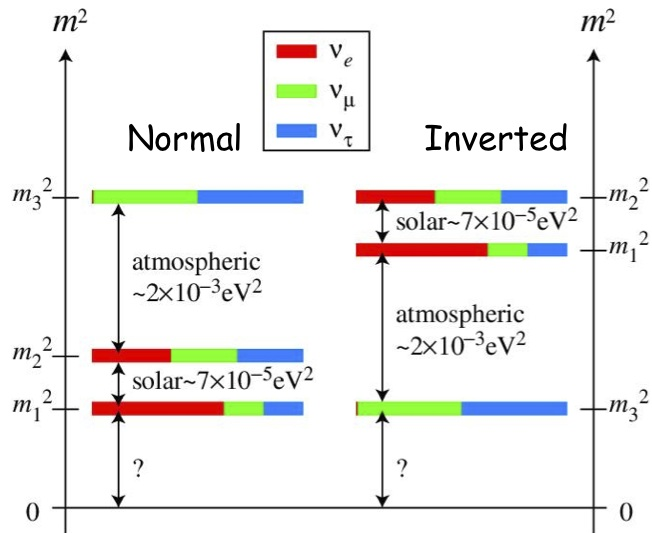
\includegraphics{hierarchy.jpg}
    \caption{Pictorial view of current results}
    \label{hierarchy}
\end{figure}\\
\noindent
The hierarchical structure of the mass is still unknown and this is known as the \textbf{hierarchy problem}. From this, it is possible to conclude that the third mixing angle $\theta_{13}$ which is the amount of $\nu_e$ in the \nth{3} state is much smaller compared to the other two mixing angles.\\
The \textbf{Daya Bay experiment} consists of eight detectors, clustered in three locations within 1.9 km of six nuclear reactors. Each detector consists of 20 tons of liquid scintillator surrounded by PMTs. The experiment is designed to measure the mixing angle $\theta_{13}$ using anti-neutrinos produced in the nearby reactors, obtaining $\theta_{13}\neq0$:
\[
\sin^2(2\theta_{13})=0.084\pm0.005\Rightarrow \theta_{13}\approx8^\circ
\]
Considering now the three families, the mixing matrix $U$ becomes a $3\times3$ complex matrix with 18 parameters, 9 real ones and 9 phases. However, there are some constraints which reduce these degrees of freedom:
\[
\begin{aligned}
&\bullet \sum_i|U_{\alpha i}|^2=1 &&\text{removes 3 real parameters}\\
&\bullet \sum_iU_{\alpha i}U_{\beta i}^*=0 &&\text{removes 3 real parameters and 3 phases}\\
&\bullet \ket{\nu_\alpha}\to e^{i\varphi}\ket{\nu_\alpha} &&\text{removes 5 phases}
\end{aligned}
\]
At the end of the day we are left with three real parameters identified with the mixing angles $\theta_{12}, \theta_{13}, \theta_{23}$ and one phase $\delta$. $U$ is usually written in the following form:
\[
U=\begin{pmatrix}
    1 & 0 & 0\\
    0 & c_{23} & s_{23}\\
    0 & -s_{23} & c_{23}
\end{pmatrix}
\begin{pmatrix}
    c_{13} & 0 & s_{13}e^{-i\delta}\\
    0 & 1 & 0\\
    -s_{13}e^{+i\delta} & 0 & c_{13}
\end{pmatrix}
\begin{pmatrix}
    c_{12} & s_{12} & 0\\
    -s_{12} & c_{12} & 0\\
    0 & 0 & 1
\end{pmatrix}
\]
The phase $\delta$ is responsible for \textbf{CP violation} and it is crucial to have oscillation between three families. CP violation means that:
\[
p(\nu_\alpha\to\nu_\beta)\neq p(\overline{\nu}_\alpha\to\overline{\nu}_\beta)
\]
If $\theta_{13}$ was zero, the matrix in the middle would reduce to the identity and we would have mixing between just two families, making it impossible to have CP violation. If this was the case, we would then have (sizes of the boxes represent the probability of oscillating into one family or another):
\[
\left\{
\begin{aligned}
&\nu_\alpha\to\begin{tabular}{|p{0.8cm}|p{0.7cm}|}
\hline
    $\nu_\alpha$ & $\nu_\beta$ \\
    \hline
\end{tabular}\\
&\overline{\nu}_\alpha\to\begin{tabular}{|p{0.8cm}|p{0.7cm}|}
\hline
    $\overline{\nu}_\alpha$ & $\overline{\nu}_\beta$ \\
    \hline
\end{tabular}
\end{aligned}
\right.
\]
From CPT conservation we get:
\[
p(\nu_\alpha\to\nu_\alpha)=p(\overline{\nu}_\alpha\to\overline{\nu}_\alpha)
\]
Since we are working with two families, it follows that:
\[
p(\nu_\alpha\to\nu_\beta)=p(\overline{\nu}_\alpha\to\overline{\nu}_\beta)
\]
Therefore, with two families we cannot have CP violation. Let's look now at the case with three families:
\[
\left\{
\begin{aligned}
&\nu_\alpha\to\begin{tabular}{|p{0.5cm}|p{0.5cm}|p{0.5cm}|}
\hline
    $\nu_\alpha$ & $\nu_\beta$ & $\nu_\gamma$\\
    \hline
\end{tabular}\\
&\overline{\nu}_\alpha\to\begin{tabular}{|p{0.5cm}|p{0.35cm}|p{0.65cm}|}
\hline
    $\overline{\nu}_\alpha$ & $\overline{\nu}_\beta$ & $\overline{\nu}_\gamma$ \\
    \hline
\end{tabular}
\end{aligned}
\right.
\]
In this case, it might be possible that $p(\nu_\alpha\to\nu_\beta)\neq p(\overline{\nu}_\alpha\to\overline{\nu}_\beta)$. The amount of CP violation can be quantified:
\begin{align*}
p(\nu_\alpha\to\nu_\beta)-p(\overline{\nu}_\alpha\to\overline{\nu}_\beta)&=\sum_{jk}U_{\alpha j}U_{\beta j}U_{\alpha k}^*U_{\beta k}^*\exp{-i\frac{\Delta m^2L}{4E}}-\sum_{jk}(\text{h.c.})\exp{-i\frac{\Delta m^2L}{4E}}\\
&=\sum_{jk}2\underbrace{\mathfrak{Im}[U_{\alpha j}U_{\beta j}U_{\alpha k}^*U_{\beta k}^*]}_{\text{Jarlskog invariant}}\exp{-i\frac{\Delta m^2L}{4E}}
\end{align*}
The \textbf{Jarlskog invariant} measures the amount of CP violation and it is parametrized as:
\[
J=c_{12}s_{12}c_{23}s_{23}c_{13}^2s_{13}\sin(\delta)
\]
Summarizing, what we know about neutrinos is that we have three families and that the flavour eigenstates are different than the mass eigenstates. Moreover, from measurements we know the mixing angles, $\Delta m^2_{12}$ and $|\Delta m^2_{13}|$. What we do not know about neutrinos is the hierarchy of their masses and whether they are a Dirac or Majorana particle, i.e. if neutrinos are their own anti-particle or not.\\
The \textbf{JUNO experiment} in China aims to determine the neutrino mass hierarchy and perform precise measurements on the mixing matrix elements. The main detector consist of 20000 tons of liquid scintillator surrounded by more than 50000 PMTs located 700 m underground. The larger distance from reactors (compared to the Daya Bay experiment) makes it better able to distinguish between neutrino oscillations. The main approach of this detector is the observation of $\overline{\nu}_e$ coming from two nuclear plants. The expected rate of neutrinos reaching the detector is known, therefore the absence of a certain neutrino flavour can give indication of oscillations.\\
In the case neutrinos are Dirac particles, it is possible to switch from left- to right-handed and vice-versa with a Lorentz transformation (LT) and to their respective anti-particle with a CPT transformation.
\begin{center}
\begin{tikzpicture}[
%roundnode/.style={circle, draw=green!60, fill=green!5, very thick, minimum size=7mm},
%squarednode/.style={rectangle, draw=red!60, fill=red!5, very thick, minimum size=5mm},
]
%Nodes
\node(nuL) {$\nu_L$};
\node(antinuR)[below=of nuL] {$\overline{\nu}_R$};
\node(nuR)[right=of nuL] {$\nu_R$};
\node(antinuL)[below=of nuR] {$\overline{\nu}_L$};

%Lines
\draw[<->] (antinuR.north) -- (nuL.south) node [pos=0.5,left] {\footnotesize CPT};
\draw[<->] (nuL.east) -- (nuR.west) node [pos=0.5,above] {\footnotesize LT};
\draw[<->] (nuR.south) -- (antinuL.north) node [pos=0.5,right] {\footnotesize CPT};
\draw[<->] (antinuR.east) -- (antinuL.west) node [pos=0.5,below] {\footnotesize LT};
\end{tikzpicture}
\end{center}
This is a Dirac neutrino, we have 4 states. However, neutrinos does not have a charge, they behave more like neutrons. Neutrinos have a lepton number which is not conserved in the Standard Model, so it can be possible to perform a simple change from left- to right-handed neutrinos.\\
Majorana tackles the problem of reformulating the Dirac theory without the problems connected to the idea of negative energy states, underlining the non-existence for some particles of their respective anti-particles. Basic transitions of the Fermi theory are:
\[
n\to p+e^-+\overline{\nu}_e \quad p\to n+e^++\nu_e
\]
Neutrinos emitted in these two processes have different helicity, which might in principle be the two spin states predicted by Majorana, which requires $\nu=\overline{\nu}$.
\begin{center}
\begin{tikzpicture}
\node(nuL) {$\nu_L$};
\node(nuR)[right=of nuL] {$\nu_R$};
\node(e-)[below=of nuL] {$e^-$};
\node(e+)[below=of nuR] {$e^+$};

\draw[<->] (nuL.east) -- (nuR.west);
\draw[->] (nuL.south) -- (e-.north) node [pos=0.5, left] {\footnotesize{emits}};
\draw[->] (nuR.south) -- (e+.north) node [pos=0.5, right] {\footnotesize{emits}};
\end{tikzpicture}
\end{center}
The particle emitted with $e^-$ has positive helicity. If neutrinos have mass, then $\nu\to e^-$ is dominant with respect to $\nu\to e^+$. Theories are pushing in favour of the Majorana hypothesis but there is no experimental evidence for that.\\
The only process in which it is possible to distinguish between Majorana and Dirac neutrinos is \textbf{double beta-decay without neutrinos}, $\beta\beta0\nu$. Neutrinos are produced in weak decays, which normally produce one electron/positron, emit a neutrino/anti-neutrino and increase the nucleus' proton number by one. There are a number of elements that cannot emit \textit{only} one electron and can decay only by emitting two electrons.
\[
(A,Z)\to(A,Z+2)+2e^-+2\overline{\nu}_e
\]
This can happen in some even-even nuclei where a single beta decay is energetically forbidden. Two beta decays are allowed, but a simultaneous decay of two nucleons in the same nucleus is extremely unlikely, the experimentally observed lifetimes of such decay processes are in the range $10^{18}-10^{21}$ years. The Feynman diagrams for such process are the following:
\begin{center}
\begin{tikzpicture}
  \begin{feynman}
  \vertex (i1) {$n$};
  \vertex [below=3.5cm of i1] (i2) {$n$};
  \vertex [right=of i1] (v1);
  \vertex [right=of i2] (v2);
  \vertex [right=of v1] (f1) {$p$};
  \vertex [right=of v2] (f2) {$p$};
  \vertex [below right=1cm of v1] (v11);
  \vertex [above right=1cm of v2] (v22);
  \vertex [right=of v11] (e1) {$e^-$};
  \vertex [right=of v22] (e2) {$e^-$};
  \vertex [below right=0.75cm of v11] (nu1) {$\overline{\nu}_e$};
  \vertex [above right=0.75cm of v22] (nu2) {$\overline{\nu}_e$};
    % \vertex (b);
    % \vertex [below=of b] (c);
    % \vertex [below left=1cm and 0.4cm of c] (d);
    % \vertex [above left=1cm and 0.4cm of b] (a);
    % \vertex [left=of a] (i1) {$n$};
    % \vertex [left=of d] (i2) {$n$};
    % \vertex[above right of=a] (f1) {$p$};
    % \vertex[right of=b] (f2) {$e^-$};
    % \vertex[right of=c] (f3) {$e^-$};
    % \vertex[below right of=d] (f4) {$p$};

    \diagram* {
    (i1) -- [fermion] (v1) -- [fermion] (f1),
    (i2) -- [fermion] (v2) -- [fermion] (f2),
    (v1) -- [photon, edge label'=$W$] (v11),
    (v2) -- [photon,edge label=$W$] (v22),
    (v11) -- [fermion] (e1),
    (v22) -- [fermion] (e2),
    (nu1) -- [fermion] (v11),
    (nu2) -- [fermion] (v22),
      % (a) -- [photon, edge label=$W$] (b) -- [majorana, insertion=0.5, edge label=$\nu_M$] (c) -- [photon, edge label=$W$] (d) ,
      % (i1) -- [fermion] (a),
      % (i2) -- [fermion] (d),
      % (a) -- [fermion] (f1),
      % (b) -- [fermion] (f2),
      % (c) -- [fermion] (f3),
      % (d) -- [fermion] (f4),
    };
  \end{feynman}
\end{tikzpicture}
\end{center}
If neutrinos are their own anti-particle, the two neutrino lines in the diagram above can be connected. In other words, the neutrino emitted in the decay of the first neutron can be absorbed by the second neutron. This leads to neutrinoless double beta decay:
\[
(A,Z)\to(A,Z+2)+2e^-
\]
$\beta\beta0\nu$ can only occur if neutrinos are Majorana particles and if neutrinos can change between left- and right-handed chirality between emission and absorption, i.e. between the two W vertices, which is possible for a non-zero neutrino mass.
\begin{center}
\begin{tikzpicture}
  \begin{feynman}
    \vertex (b);
    \vertex [below=of b] (c);
    \vertex [below left=1cm and 0.4cm of c] (d);
    \vertex [above left=1cm and 0.4cm of b] (a);
    \vertex [left=of a] (i1) {$n$};
    \vertex [left=of d] (i2) {$n$};
    \vertex[above right of=a] (f1) {$p$};
    \vertex[right of=b] (f2) {$e^-$};
    \vertex[right of=c] (f3) {$e^-$};
    \vertex[below right of=d] (f4) {$p$};

    \diagram* {
      (a) -- [photon, edge label=$W$] (b) -- [majorana, insertion=0.5, edge label=$\nu_M$] (c) -- [photon, edge label=$W$] (d) ,
      (i1) -- [fermion] (a),
      (i2) -- [fermion] (d),
      (a) -- [fermion] (f1),
      (b) -- [fermion] (f2),
      (c) -- [fermion] (f3),
      (d) -- [fermion] (f4),
    };
  \end{feynman}
\end{tikzpicture}
\end{center}
This is called \textbf{matter creation} because it is a process which \textit{favour} creation of matter instead of anti-matter. The cross in the diagram corresponds to the \textbf{chirality flip} which is proportional to $m^2_{\beta\beta}=|\sum_jU_{ej}^2m_j|^2$ and it depends on the effective Majorana neutrino mass.\\
The \textbf{CUORE experiment} is currently investigating $\beta\beta0\nu$ in $^{130}$Te. It uses 742 kg of TeO$_2$ crystals ($\sim$246 kg of $^{130}$Te) and it looks for peaks around the known decay energy of $^{130}$Te of $Q\approx2.5$\,MeV.
\end{document}